\section{HỆ THỐNG SỐ ĐẾM - SỐ NHỊ PHÂN}
\subsection{Các hệ thống số đếm:}
\subsubsection{Khái niệm:}
\begin{itemize}
    \item[-] Cơ số (r-radix): là số lượng ký tự chữ số (ký số - digit) sử dụng để biểu diễn trong hệ thống số đếm.
    \item[-] Trọng số (weight): đại lượng biểu diễn cho vị trí của 1 con số trong chuỗi số.\\ \textbf{Trọng số = $\text{Cơ số}^\text{vị trí}$}
    \item[-] Giá trị (value): tính bằng tổng theo trọng số. \textbf{Giá trị = $\sum$ (Ký số $\times$ Trọng số).}
\end{itemize}
\textbf{a. Số thập phân (Decimal): Cơ số $r = 10$.}
\begin{table}[h!]
    \centering
    \begin{tabular}{|c|c|c|c|c|c|c|}
    \hline
    \textbf{4}                                   & \textbf{0}                                   & \textbf{7}                                   & \textbf{.} & \textbf{6}                                        & \textbf{2}                                        & \textbf{5}                                        \\ \hline
    $10^2$                        & $10^1$                        & $10^0$                        & .          & $10^{-1} $                       & $10^{-2}$                        & $10^{-3}$                        \\ 
    $4\times 10^2$ & $0\times 10^1$ & $7\times 10^0$ & .          & $6\times 10^{-1}$ & $2\times 10^{-2}$ & $5\times 10^{-3}$ \\ 
   $ 400 $                                         & $0$                                            & $7$                                            & .          & $0.6$                                               & $0.02$                                              & $0.005$                                             \\ \hline
    \end{tabular}
\end{table}
\[
    400 + 0 + 7 + 0.6 + 0.02 + 0.005 = 407.625
\]
\textbf{b. Số nhị phân (Binary): Cơ số $r=2$.}
\begin{table}[h!]
    \centering
    \begin{tabular}{|c|c|c|c|c|c|c|}
    \hline
    \textbf{1}                                   & \textbf{0}                                   & \textbf{1}                                   & \textbf{.} & \textbf{0}                                        & \textbf{1}                                        & \textbf{1}                                        \\ \hline
    $2^2$                        & $2^1$                        & $2^0$                        & .          & $2^{-1} $                       & $2^{-2}$                        & $2^{-3}$                        \\ 
    $1\times 2^2$ & $0\times 2^1$ & $1\times 2^0$ & .          & $0\times 2^{-1}$ & $1\times 2^{-2}$ & $1\times 2^{-3}$ \\ 
   $ 4 $                                         & $0$                                            & $1$                                            & .          & $0$                                               & $0.25$                                              & $0.125$                                             \\ \hline
    \end{tabular}
\end{table}
\[
    4 + 0 +1+0+0.25+0.125=5.375
\]
\textbf{c. Số thập lục phân (Hexadecimal): Cơ số $r=16$}
\begin{table}[h!]
    \centering
    \begin{tabular}{|c|c|c|c|c|c|c|}
    \hline
    \textbf{5}     & \textbf{A}      & \textbf{0}     & \textbf{.} & \textbf{4}        & \textbf{D}         & \textbf{1}        \\ \hline
    $16^2$         & $16^1$          & $16^0$         & .          & $16^{-1} $        & $16^{-2}$          & $16^{-3}$         \\ 
    $5\times 16^2$ & $10\times 16^1$ & $0\times 16^0$ & .          & $4\times 16^{-1}$ & $13\times 16^{-2}$ & $1\times 16^{-3}$ \\ 
    $ 1280 $       & $160$           & $0$            & .          & $0.25$            & $0.0508$           & $0.002$           \\ \hline
    \end{tabular}
\end{table}
\[
    1280 + 160+0+0.25+0.0508+0.0002 = 1440.301
\]
\subsubsection{Chuyển đổi cơ số:}
\noindent\textbf{a. Từ thập phân sang nhị phân:}
\newpage
\[
  8.625  
\]
\begin{center}
    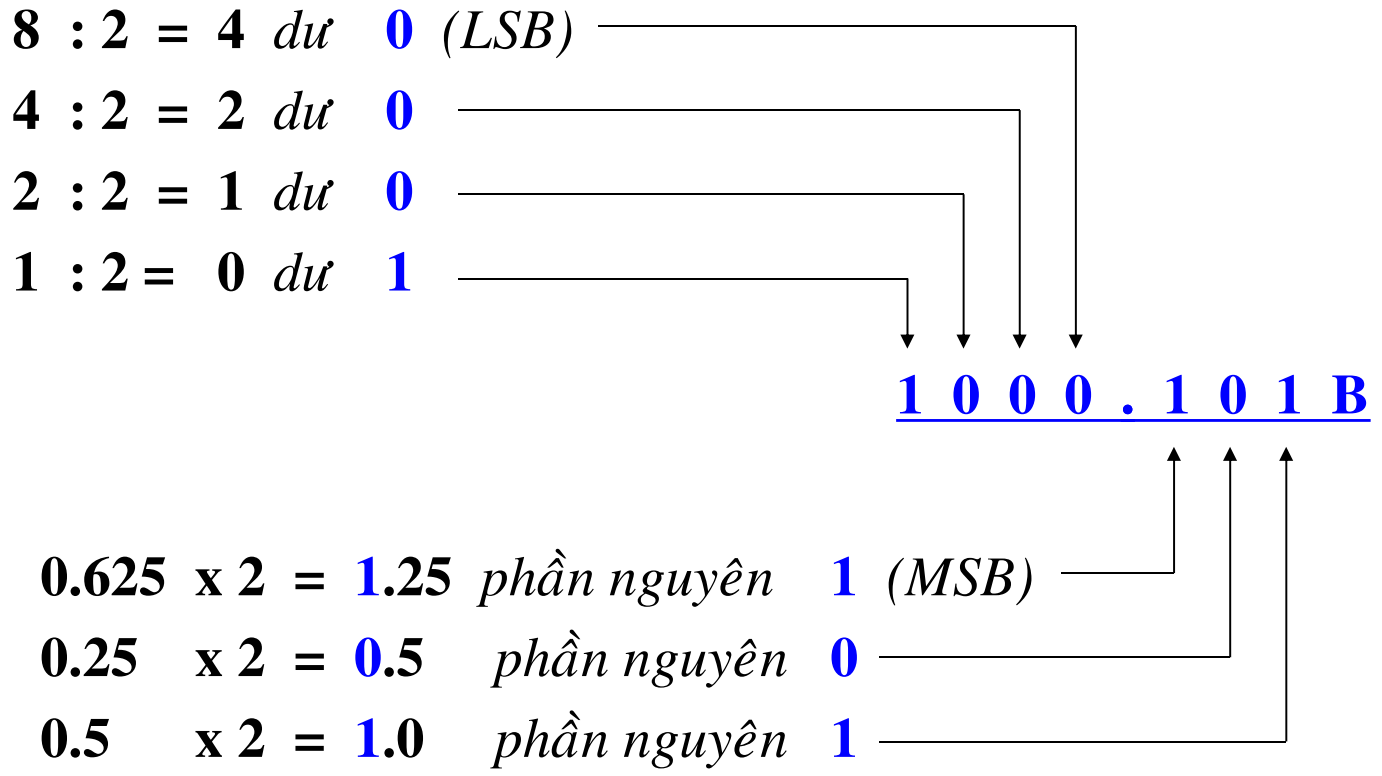
\includegraphics[width = 0.65\textwidth]{./local/image/1.png}
\end{center}
Ta lấy phần nguyên chia cho 2 và dừng khi ta được 0 dư 1, phần không nguyên nhân với cơ số 2 và giữ phần nguyên, tiếp tục cho tới khi có phần không nguyên là 0.

\noindent\textbf{b. Từ thập phân sang thập lục phân:}
\[
    1480.4296875
\]
\begin{center}
    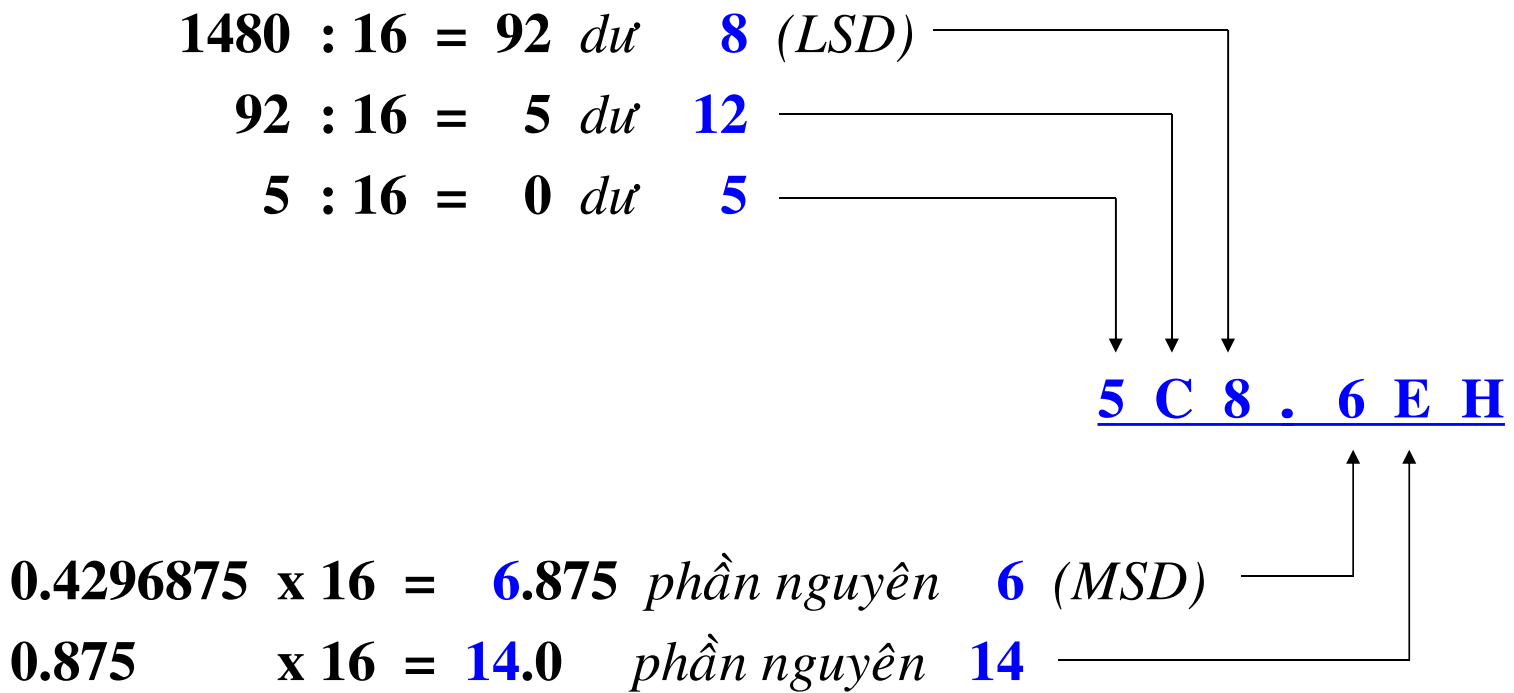
\includegraphics[width = 0.65\textwidth]{./local/image/2.png}
\end{center}
\textbf{c. Từ nhị phân sang thập lục phân}
\begin{center}
    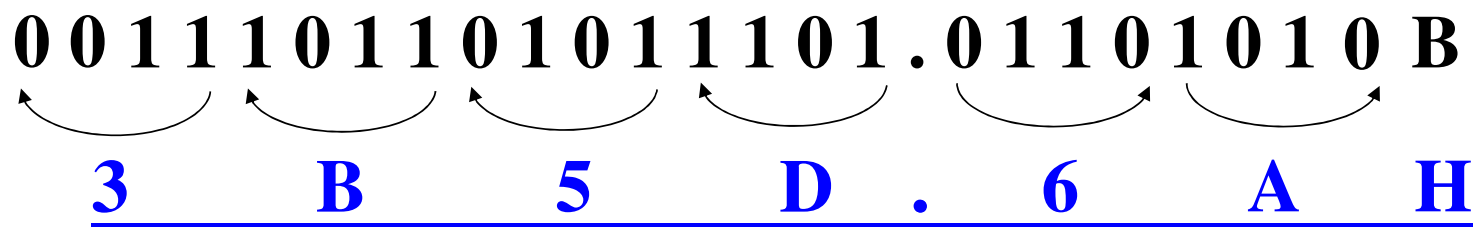
\includegraphics[width = 0.65\textwidth]{./local/image/3.png}
\end{center}
\textbf{d. Từ thập lục phân sang nhị phân}
\begin{center}
    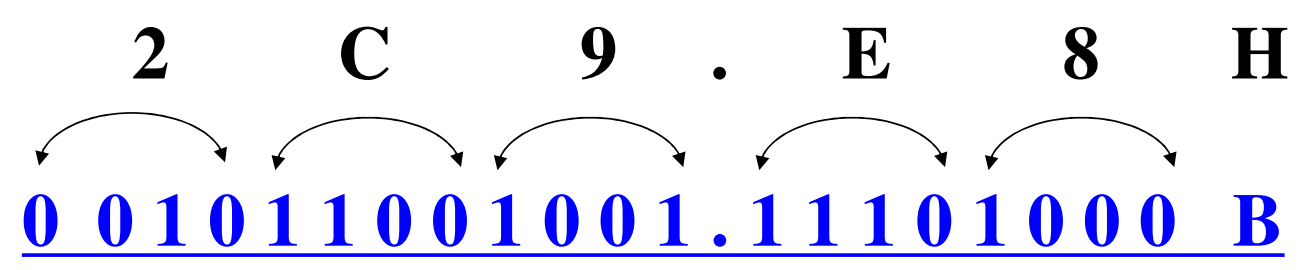
\includegraphics[width = 0.65\textwidth]{./local/image/4.png}
\end{center}
\subsection{Số nhị phân (Binary):}
\subsubsection{Các tính chất của số nhị phân}
\begin{itemize}
    \item[-] Số nhị phân n bit có $2^n$ giá trị từ $0$ đến $2^n-1$.
    \item[-] Số nhị phân có giá trị $2^n-1$: $1\cdots \cdots \cdots 1$ (n bit 1) và giá trị $2^n$: $1 \ 0 \cdots \cdots \cdots 0$ (n bit 0).
    \item[-] Số nhị phân có giá trị lẻ là số có LSB = 1; ngược lại giá trị chẵn là số có LSB = 0.
    \item[-] Các bội số của bit:
\end{itemize}
\begin{center}
    1 B (Byte) = 8 bit \\
    1 KB = $2^{10}$ B \\
    1 MB = $2^{10}$ KB \\
    1 GB = $2^{10}$ MB 
\end{center}
\subsubsection{Các phép toán số học trên số nhị phân:}
\noindent\textbf{a. Phép cộng}
\begin{center}
    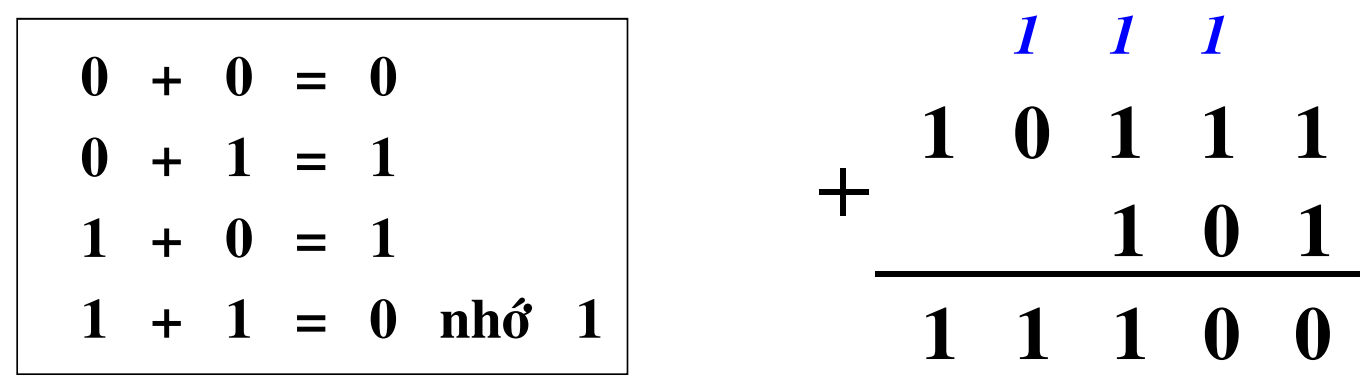
\includegraphics[width = 0.65\textwidth]{./local/image/5.png}
\end{center}
\textbf{b. Phép trừ}
\begin{center}
    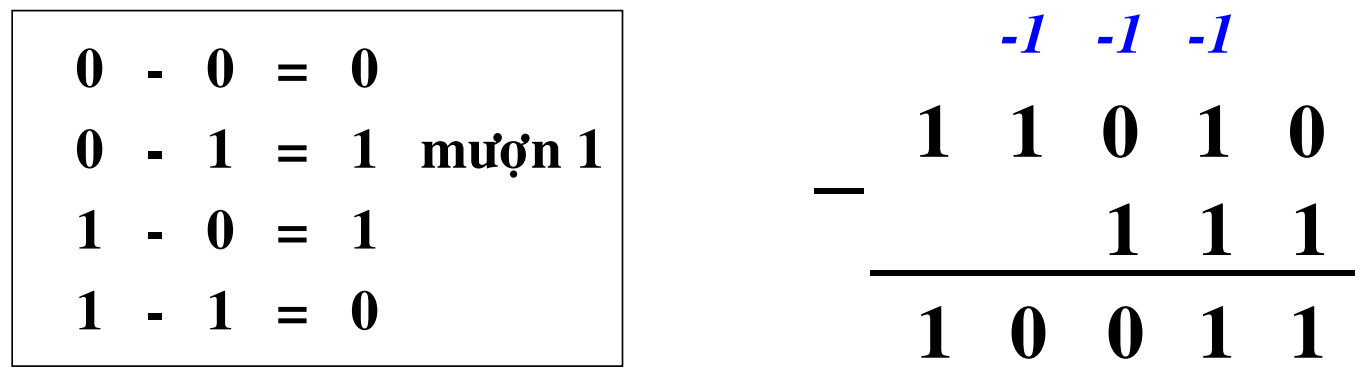
\includegraphics[width = 0.65\textwidth]{./local/image/6.png}
\end{center}
\textbf{c. Phép nhân}
\begin{center}
    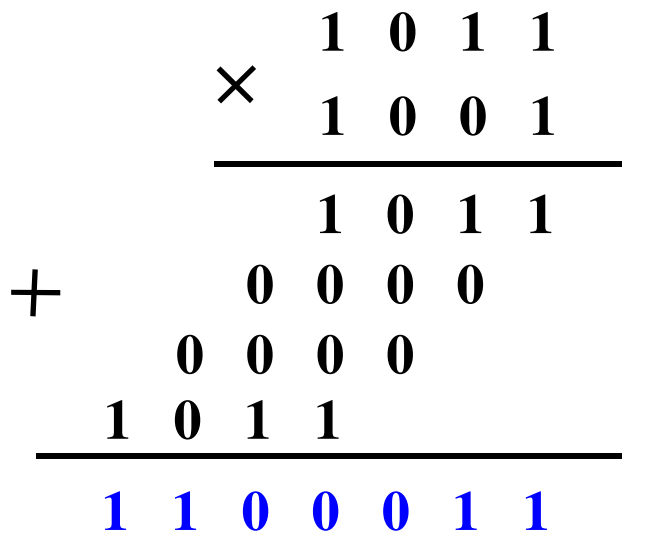
\includegraphics[width = 0.35\textwidth]{./local/image/7.png}
\end{center}
\textbf{d. Phép chia}
\begin{center}
    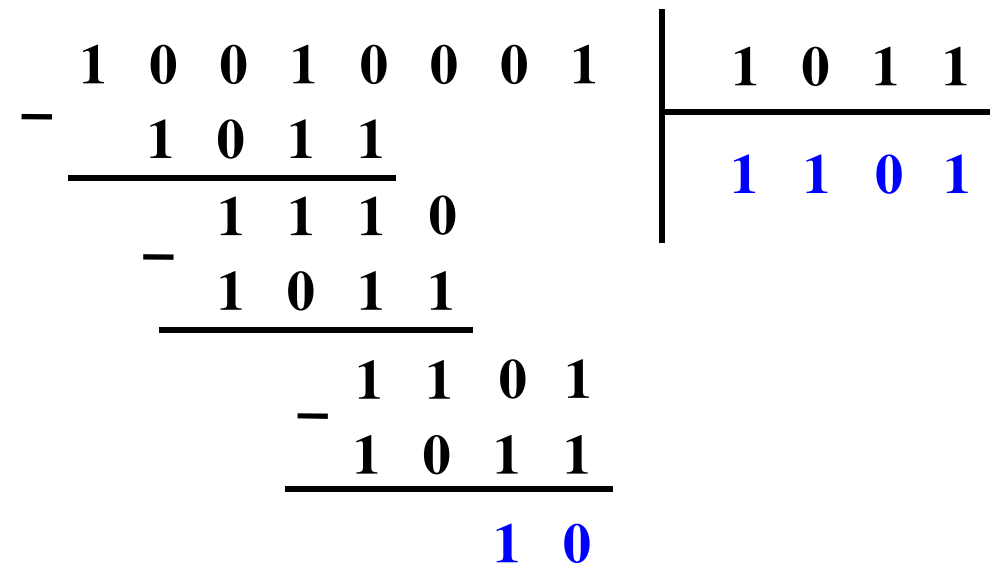
\includegraphics[width = 0.45\textwidth]{./local/image/8.png}
\end{center}
\subsubsection{Mã nhị phân:}
\textit{\textbf{Từ mã:}} là các tổ hợp nhị phân được sử dụng trong loại mã nhị phân.\\
\textbf{a. Mã nhị phân cho số thập phân (BCD - Binary Coded Decimal)}
\begin{table}[h!]
    \centering
    \begin{tabular}{|c|c|c|c|c|}
    \hline
    \textbf{\begin{tabular}[c]{@{}c@{}}Số\\ thập phân\end{tabular}} & \textbf{\begin{tabular}[c]{@{}c@{}}BCD\\ (8 4 2 1)\end{tabular}} & \textbf{\begin{tabular}[c]{@{}c@{}}BCD\\ (2 4 2 1)\end{tabular}} & \textbf{\begin{tabular}[c]{@{}c@{}}BCD\\ quá 3\end{tabular}} & \textbf{Mã 1 trong 10} \\ \hline
    0                                                               & 0000                                                             & 0000                                                             & 0011                                                         & 0000000001             \\ 
    1                                                               & 0001                                                             & 0001                                                             & 0100                                                         & 0000000010             \\ 
    2                                                               & 0010                                                             & 0010                                                             & 0101                                                         & 0000000100             \\ 
    3                                                               & 0011                                                             & 0011                                                             & 0110                                                         & 0000001000             \\ 
    4                                                               & 0100                                                             & 0100                                                             & 0111                                                         & 0000010000             \\ 
    5                                                               & 0101                                                             & 1011                                                             & 1000                                                         & 0000100000             \\ 
    6                                                               & 0110                                                             & 1100                                                             & 1001                                                         & 0001000000             \\ 
    7                                                               & 0111                                                             & 1101                                                             & 1010                                                         & 0010000000             \\ 
    8                                                               & 1000                                                             & 1110                                                             & 1011                                                         & 0100000000             \\ 
    9                                                               & 1001                                                             & 1111                                                             & 1100                                                         & 1000000000             \\ \hline
    \end{tabular}
\end{table}\\
\textbf{b. Mã Gray:} là mã nhị phân mà 2 giá trị liên tiếp nhau có tổ hợp bit biểu diễn chỉ khác nhau 1 bit.
\begin{table}[h!]
    \centering
    \begin{tabular}{|c|c|c|}
    \hline
    \textit{\textbf{Giá trị}} & \textit{\textbf{Binary}} & \textit{\textbf{Gray}} \\ \hline
    0                         & 000                      & 000                    \\ 
    1                         & 001                      & 001                    \\ 
    2                         & 010                      & 011                    \\ 
    3                         & 011                      & 010                    \\ 
    4                         & 100                      & 110                    \\ \hline
    \end{tabular}
\end{table}
\begin{center}
    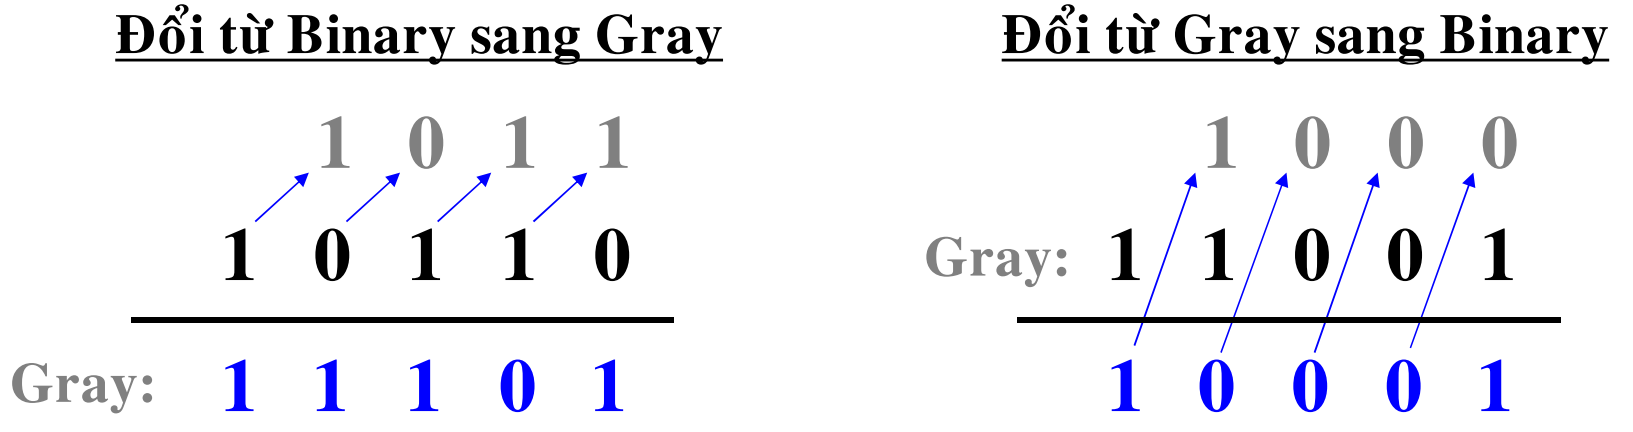
\includegraphics[width = 0.9\textwidth]{./local/image/9.png}
\end{center}
\textbf{c. Mã LED 7 đoạn}
\begin{center}
    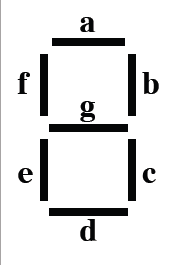
\includegraphics[width = 0.2\textwidth]{./local/image/16.png} \qquad \qquad \qquad \qquad 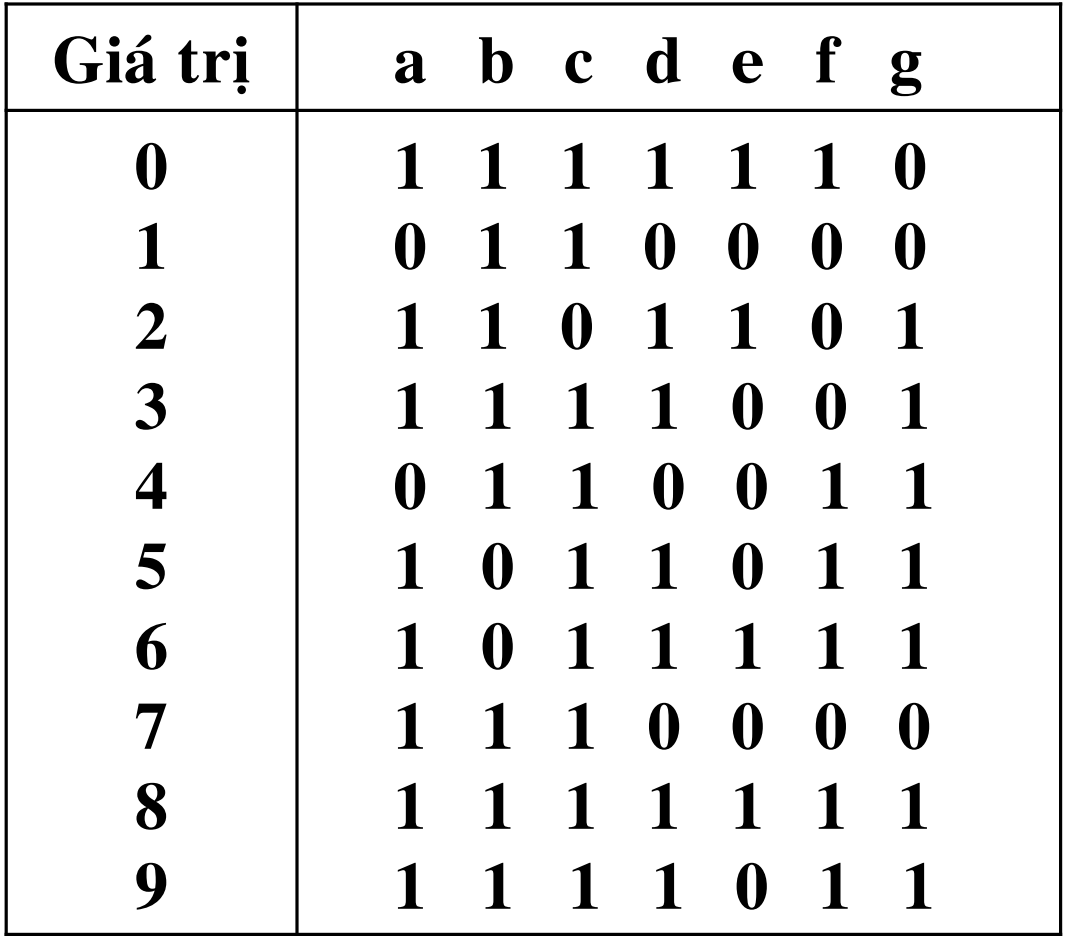
\includegraphics[width = 0.45\textwidth]{./local/image/17.png}
\end{center}
\textbf{d. Mã 1 trong n:} là mã nhị phân n bit có mỗi từ mã chỉ có 1 bit là 1 (hoặc 0) và n-1 bit còn lại là 0 (hoặc 1).
\begin{center}
    
\includegraphics[width = 0.7\textwidth]{./local/image/18.png}
\end{center}
\textbf{e. Mã ký tự ASCII:}
% Please add the following required packages to your document preamble:
% \usepackage[table,xcdraw]{xcolor}
% Beamer presentation requires \usepackage{colortbl} instead of \usepackage[table,xcdraw]{xcolor}
\begin{table}[h!]
    \centering
    \begin{tabular}{|c|c|cccccccc|}
    \hline
                   &                            & \multicolumn{8}{c|}{(Cột) $b_6b_5b_4$}                                                                                                                                                                                                                                                                                                                                   \\ \hline
    (Hàng)         &                            & \multicolumn{1}{c|}{000}                      & \multicolumn{1}{c|}{001}                      & \multicolumn{1}{c|}{010}                      & \multicolumn{1}{c|}{011}                      & \multicolumn{1}{c|}{100}                      & \multicolumn{1}{c|}{101}                      & \multicolumn{1}{c|}{110}                      & 111                      \\ \hline
    $b_3b_2b_1b_0$ & {\color[HTML]{0000FF} Hex} & \multicolumn{1}{c|}{{\color[HTML]{0000FF} 0}} & \multicolumn{1}{c|}{{\color[HTML]{0000FF} 1}} & \multicolumn{1}{c|}{{\color[HTML]{0000FF} 2}} & \multicolumn{1}{c|}{{\color[HTML]{0000FF} 3}} & \multicolumn{1}{c|}{{\color[HTML]{0000FF} 4}} & \multicolumn{1}{c|}{{\color[HTML]{0000FF} 5}} & \multicolumn{1}{c|}{{\color[HTML]{0000FF} 6}} & {\color[HTML]{0000FF} 7} \\ \hline
    0000           & {\color[HTML]{0000FF} 0}   & \multicolumn{1}{c|}{NUL}                      & \multicolumn{1}{c|}{DLE}                      & \multicolumn{1}{c|}{SP}                       & \multicolumn{1}{c|}{0}                        & \multicolumn{1}{c|}{@}                        & \multicolumn{1}{c|}{P}                        & \multicolumn{1}{c|}{`}                        & p                        \\ 
    0001           & {\color[HTML]{0000FF} 1}   & \multicolumn{1}{c|}{SOH}                      & \multicolumn{1}{c|}{DC1}                      & \multicolumn{1}{c|}{!}                        & \multicolumn{1}{c|}{1}                        & \multicolumn{1}{c|}{A}                        & \multicolumn{1}{c|}{Q}                        & \multicolumn{1}{c|}{a}                        & q                        \\ 
    0010           & {\color[HTML]{0000FF} 2}   & \multicolumn{1}{c|}{STX}                      & \multicolumn{1}{c|}{DC2}                      & \multicolumn{1}{c|}{"}                        & \multicolumn{1}{c|}{2}                        & \multicolumn{1}{c|}{B}                        & \multicolumn{1}{c|}{R}                        & \multicolumn{1}{c|}{b}                        & r                        \\ 
    0011           & {\color[HTML]{0000FF} 3}   & \multicolumn{1}{c|}{ETX}                      & \multicolumn{1}{c|}{DC3}                      & \multicolumn{1}{c|}{\#}                       & \multicolumn{1}{c|}{3}                        & \multicolumn{1}{c|}{C}                        & \multicolumn{1}{c|}{S}                        & \multicolumn{1}{c|}{c}                        & s                        \\ 
    0100           & {\color[HTML]{0000FF} 4}   & \multicolumn{1}{c|}{EOT}                      & \multicolumn{1}{c|}{DC4}                      & \multicolumn{1}{c|}{\$}                       & \multicolumn{1}{c|}{4}                        & \multicolumn{1}{c|}{D}                        & \multicolumn{1}{c|}{T}                        & \multicolumn{1}{c|}{d}                        & t                        \\ 
    0101           & {\color[HTML]{0000FF} 5}   & \multicolumn{1}{c|}{ENQ}                      & \multicolumn{1}{c|}{NAK}                      & \multicolumn{1}{c|}{\%}                       & \multicolumn{1}{c|}{5}                        & \multicolumn{1}{c|}{E}                        & \multicolumn{1}{c|}{U}                        & \multicolumn{1}{c|}{e}                        & u                        \\ 
    0110           & {\color[HTML]{0000FF} 6}   & \multicolumn{1}{c|}{ACK}                      & \multicolumn{1}{c|}{SYN}                      & \multicolumn{1}{c|}{\&}                       & \multicolumn{1}{c|}{6}                        & \multicolumn{1}{c|}{F}                        & \multicolumn{1}{c|}{V}                        & \multicolumn{1}{c|}{f}                        & v                        \\ 
    0111           & {\color[HTML]{0000FF} 7}   & \multicolumn{1}{c|}{BEL}                      & \multicolumn{1}{c|}{ETB}                      & \multicolumn{1}{c|}{'}                        & \multicolumn{1}{c|}{7}                        & \multicolumn{1}{c|}{G}                        & \multicolumn{1}{c|}{W}                        & \multicolumn{1}{c|}{g}                        & w                        \\ 
    1000           & {\color[HTML]{0000FF} 8}   & \multicolumn{1}{c|}{BS}                       & \multicolumn{1}{c|}{CAN}                      & \multicolumn{1}{c|}{)}                        & \multicolumn{1}{c|}{8}                        & \multicolumn{1}{c|}{H}                        & \multicolumn{1}{c|}{X}                        & \multicolumn{1}{c|}{h}                        & x                        \\ 
    1001           & {\color[HTML]{0000FF} 9}   & \multicolumn{1}{c|}{HT}                       & \multicolumn{1}{c|}{EM}                       & \multicolumn{1}{c|}{(}                        & \multicolumn{1}{c|}{9}                        & \multicolumn{1}{c|}{I}                        & \multicolumn{1}{c|}{Y}                        & \multicolumn{1}{c|}{i}                        & y                        \\ 
    1010           & {\color[HTML]{0000FF} A}   & \multicolumn{1}{c|}{LF}                       & \multicolumn{1}{c|}{SUB}                      & \multicolumn{1}{c|}{*}                        & \multicolumn{1}{c|}{:}                        & \multicolumn{1}{c|}{J}                        & \multicolumn{1}{c|}{Z}                        & \multicolumn{1}{c|}{j}                        & z                        \\ 
    1011           & {\color[HTML]{0000FF} B}   & \multicolumn{1}{c|}{VT}                       & \multicolumn{1}{c|}{ESC}                      & \multicolumn{1}{c|}{+}                        & \multicolumn{1}{c|}{;}                        & \multicolumn{1}{c|}{K}                        & \multicolumn{1}{c|}{{[}}                      & \multicolumn{1}{c|}{k}                        & \{                       \\ 
    1100           & {\color[HTML]{0000FF} C}   & \multicolumn{1}{c|}{FF}                       & \multicolumn{1}{c|}{ES}                       & \multicolumn{1}{c|}{'}                        & \multicolumn{1}{c|}{\textless{}}              & \multicolumn{1}{c|}{L}                        & \multicolumn{1}{c|}{\textbackslash{}}         & \multicolumn{1}{c|}{l}                        & |                        \\ 
    1101           & {\color[HTML]{0000FF} D}   & \multicolumn{1}{c|}{CR}                       & \multicolumn{1}{c|}{GS}                       & \multicolumn{1}{c|}{-}                        & \multicolumn{1}{c|}{=}                        & \multicolumn{1}{c|}{M}                        & \multicolumn{1}{c|}{{]}}                      & \multicolumn{1}{c|}{m}                        & \}                       \\ 
    1110           & {\color[HTML]{0000FF} E}   & \multicolumn{1}{c|}{SO}                       & \multicolumn{1}{c|}{RS}                       & \multicolumn{1}{c|}{.}                        & \multicolumn{1}{c|}{\textgreater{}}           & \multicolumn{1}{c|}{N}                        & \multicolumn{1}{c|}{\textasciicircum{}}       & \multicolumn{1}{c|}{n}                        & $\sim$                   \\ 
    1111           & {\color[HTML]{0000FF} F}   & \multicolumn{1}{c|}{SI}                       & \multicolumn{1}{c|}{US}                       & \multicolumn{1}{c|}{/}                        & \multicolumn{1}{c|}{?}                        & \multicolumn{1}{c|}{O}                        & \multicolumn{1}{c|}{\_}                       & \multicolumn{1}{c|}{o}                        & DEL                      \\ \hline
    \end{tabular}
\end{table}
\subsection{Số nhị phân có dấu:}
\subsubsection{Biểu diễn số có dấu:}
\textbf{Số có dấu theo biên độ (Signed Magnitude):}
\begin{itemize}
    \item[-] Bit MSB là bit dấu: 0 là số dương và 1 là số âm, các bit còn lại biểu diễn giá trị độ lớn.
        \[
            +13: \qquad 01101
        \]
        \[
            -13: \qquad 11101
        \]
    \item[-] Phạm vi biểu diễn:
    \[
        -(2^{n-1} - 1) \div  +(2^{n-1} - 1)
    \]
\end{itemize}
\subsubsection{Số bù 1 (1's Complement):}
\begin{itemize}
    \item[-] Số bù 1 của 1 số nhị phân N có chiều dài n bit
        \begin{center}
            Bù 1 (N) $= 2^n -1 - $N
        \end{center}
        VD: Bù 1 (1001) = $2^4$ - 1 -1001 = 1111-1001 = 0110
    \item[-] Có thể lấy Bù 1 của 1 số nhị phân bằng cách lấy đảo từng bit của nó (0 thành 1 và 1 thành 0).
\end{itemize}
\textbf{Biểu diễn số có dấu bù 1:}
\begin{itemize}
    \item[*] Số có giá trị dương: bit dấu = 0, các bit còn lại biểu diễn độ lớn.
    \item[*] Số có giá trị âm: lấy bù 1 của số dương có cùng độ lớn.
\end{itemize}
Phạm vi biểu diễn:
\[
   -(2^{n-1} - 1) \div  +(2^{n-1} - 1)
\]
\subsubsection{Số bù 2 (2's Complement):}
\begin{itemize}
    \item[-] Số bù 2 của 1 số nhị phân N có chiều dài n bit cũng có n bit
        \begin{center}
            Bù 2 (N) = $2^n - N$ = Bù 1 (N) + 1
        \end{center}
\end{itemize}
VD: Bù 2 (1001) = $2^4$ - 1001 = 10000 - 1001 = 0111. Hoặc Bù 2(1001) = Bù 1 (1001) + 1 = 0110 + 1 = 0111.

\textbf{Biểu diễn số có dấu bù 2:}
\begin{itemize}
    \item[*] Số có giá trị dương: bit dấu = 0, các bit còn lại biểu diễn độ lớn.
    \item[*] Số có giá tị âm: lấy bù 2 của số dương có cùng độ lớn.
\end{itemize}
Phạm vi biểu diễn:
    \[
        -(2^{n-1}) \div  +(2^{n-1} - 1)
    \]
\begin{table}[h!]
    \centering
    \begin{tabular}{|c|c|}
        \hline
        \textbf{Giá trị dương} & \textbf{Giá trị âm} \\ \hline
        000 = 0                & 100 = -4            \\ 
        001 = +1               & 101 = -3            \\ 
        010 = +2               & 110 = -2            \\ 
        011 = +3               & 111 = -1            \\ \hline
    \end{tabular}
\end{table}
\begin{itemize}
    \item[-] Để tìm được giá trị của só âm: ta lấy bù 2 của nó; sẽ nhận được số dương có cùng biên độ.
    \item[-] Mở rộng chiều dài bit số có dấu: số dương thêm các bit 0 và số âm thêm các bit 1 vào trước.
    \item[-] Lấy bù 2 hai lần một số thì bằng chính số đó.
    \item[-] Giá trị -1 được biểu diễn là $1/cdots11$ (n bit 1).
    \item[-] Giá trị $-2^n$ được biểu diễn là 100$/cdots$00 (n bit 0).
    \begin{center}
        -32 = -$2^5$ = 100000
    \end{center}
\end{itemize}
\subsubsection{Các phép toán cộng trừ số có dấu:}
\begin{itemize}
    \item[-] Thực hiện giống như số không dấu.
    \item[] Thực hiện trên toán hạng có cùng chiều dài bit, và kết quả cũng có cùng số bit.
    \item[] Kết quả đúng nếu nằm trong phạm vi biểu diễn số có dấu (nếu kết quả sai thì cần mở rộng chiều dài bit).
\end{itemize}
\begin{center}
    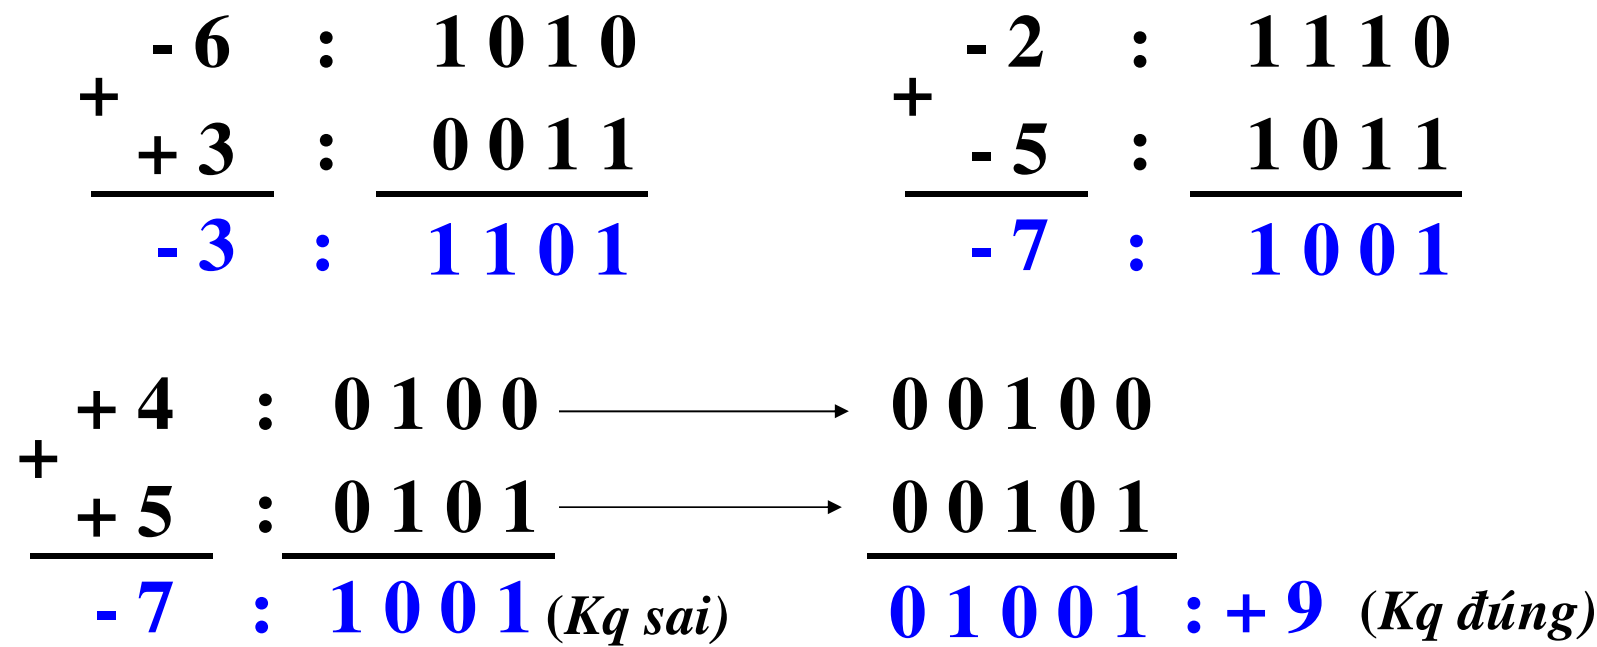
\includegraphics[width = 0.7\textwidth]{./local/image/10.png}
\end{center}
\begin{center}
    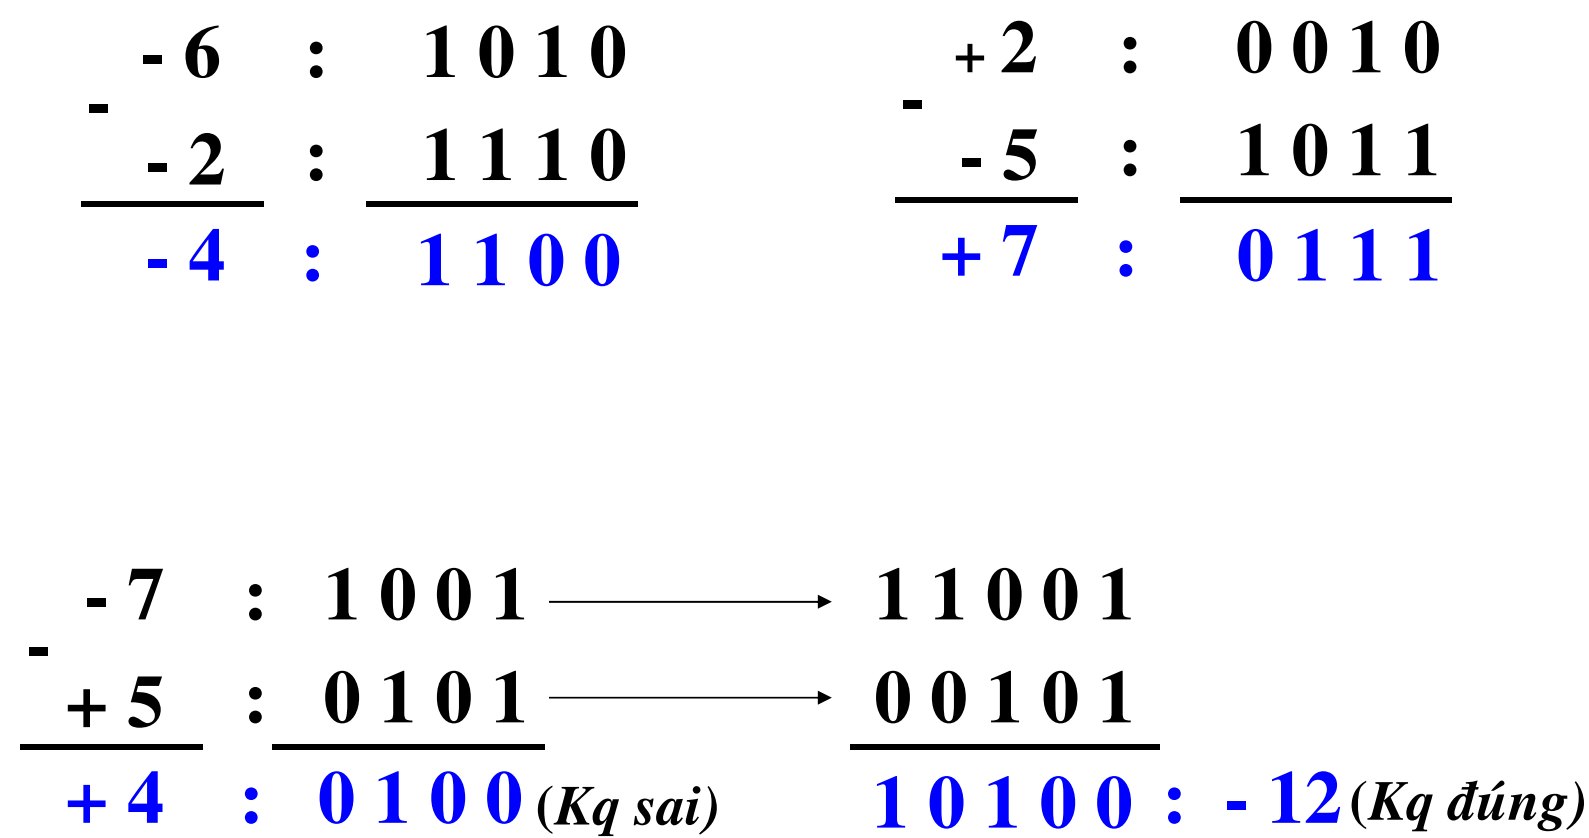
\includegraphics[width = 0.7\textwidth]{./local/image/11.png}
\end{center}
Trừ với số bù 2: A - B = A + Bù 2 (B)
\begin{itemize}
    \item Trừ với số không có dấu:
        \begin{center}
            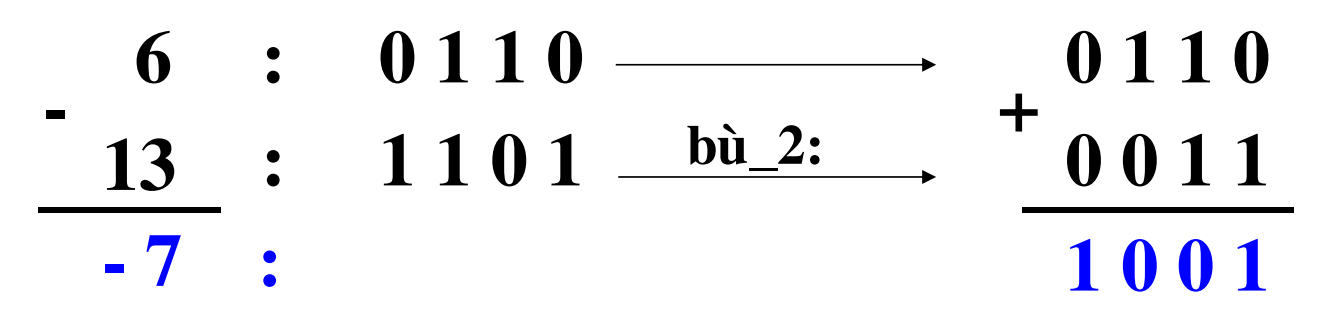
\includegraphics[width = 0.65\textwidth]{./local/image/12.png}
        \end{center}
    \item Trừ với số có dấu:
    \begin{center}
        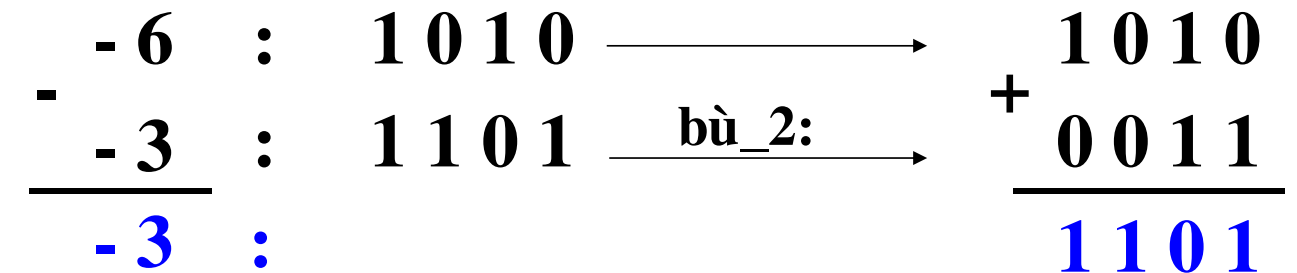
\includegraphics[width = 0.65\textwidth]{./local/image/13.png}
    \end{center}
\end{itemize}
\subsection{Cộng trừ số BCD:}
\begin{center}
    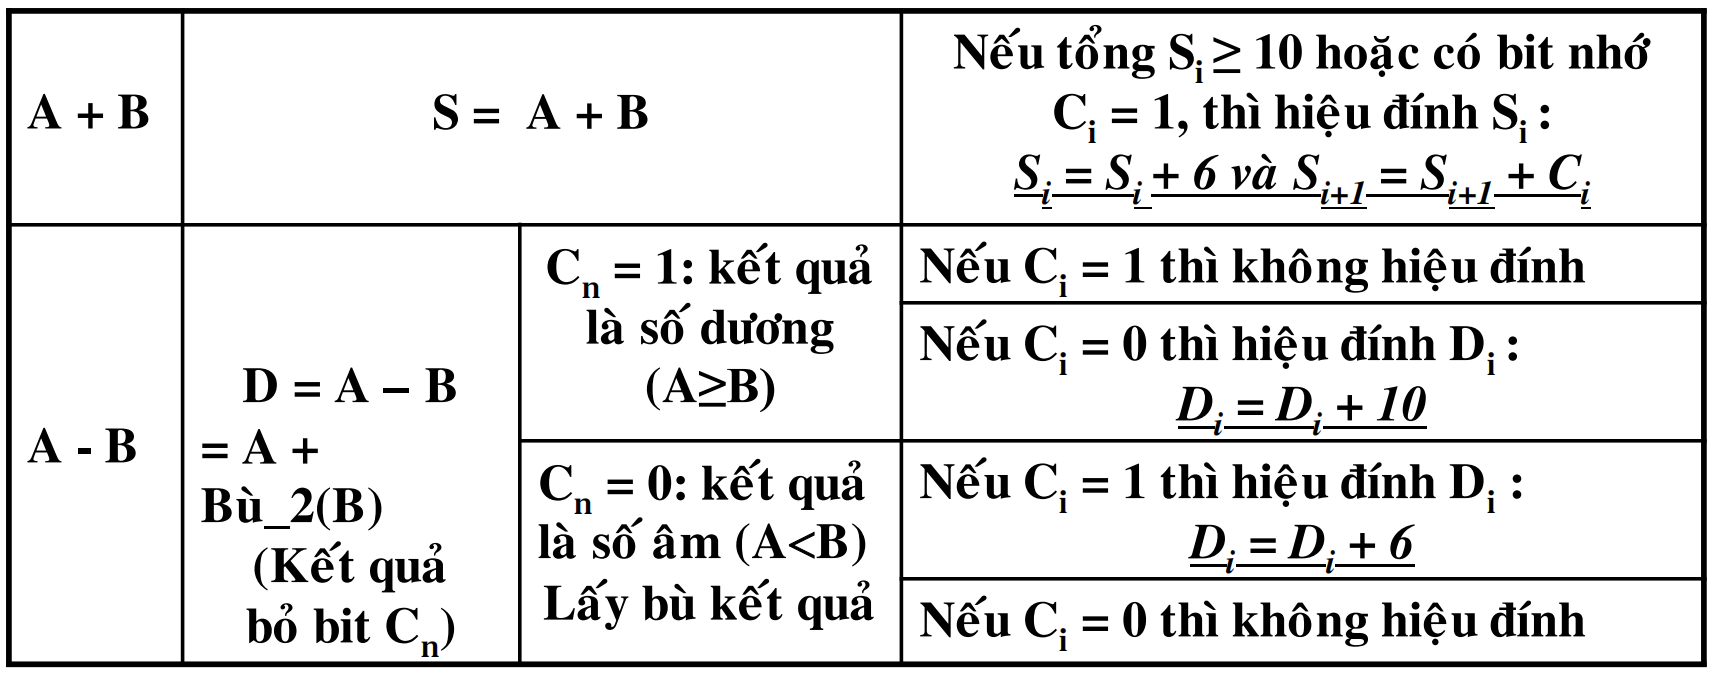
\includegraphics[width = 0.9\textwidth]{./local/image/19.png}
\end{center}
\begin{center}
    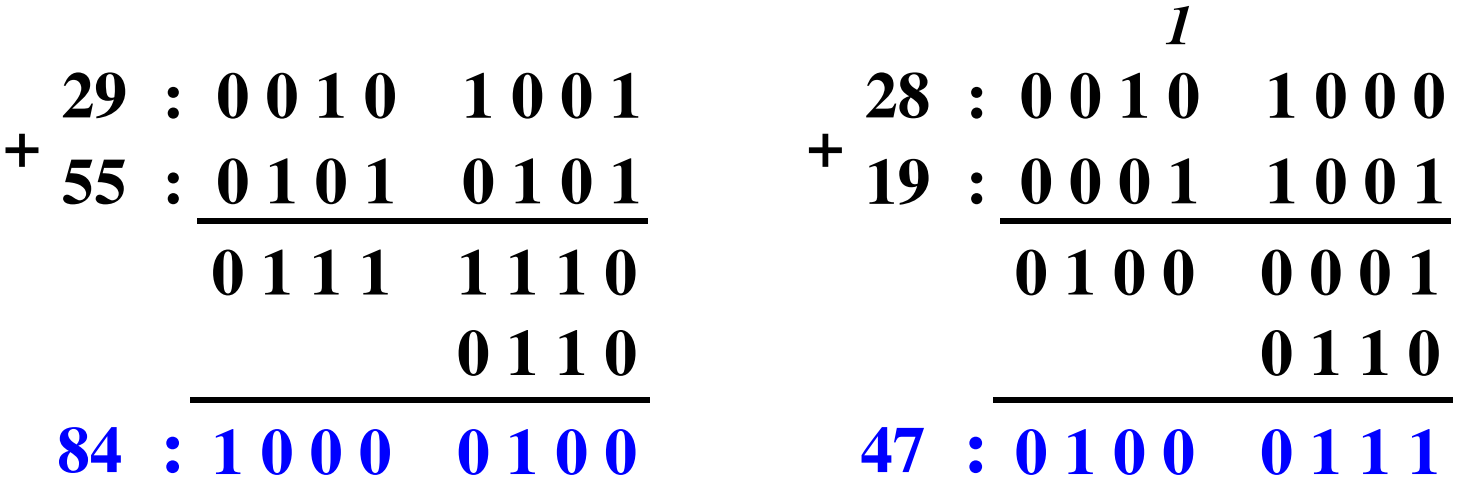
\includegraphics[width = 0.7\textwidth]{./local/image/14.png}
\end{center}
\begin{center}
    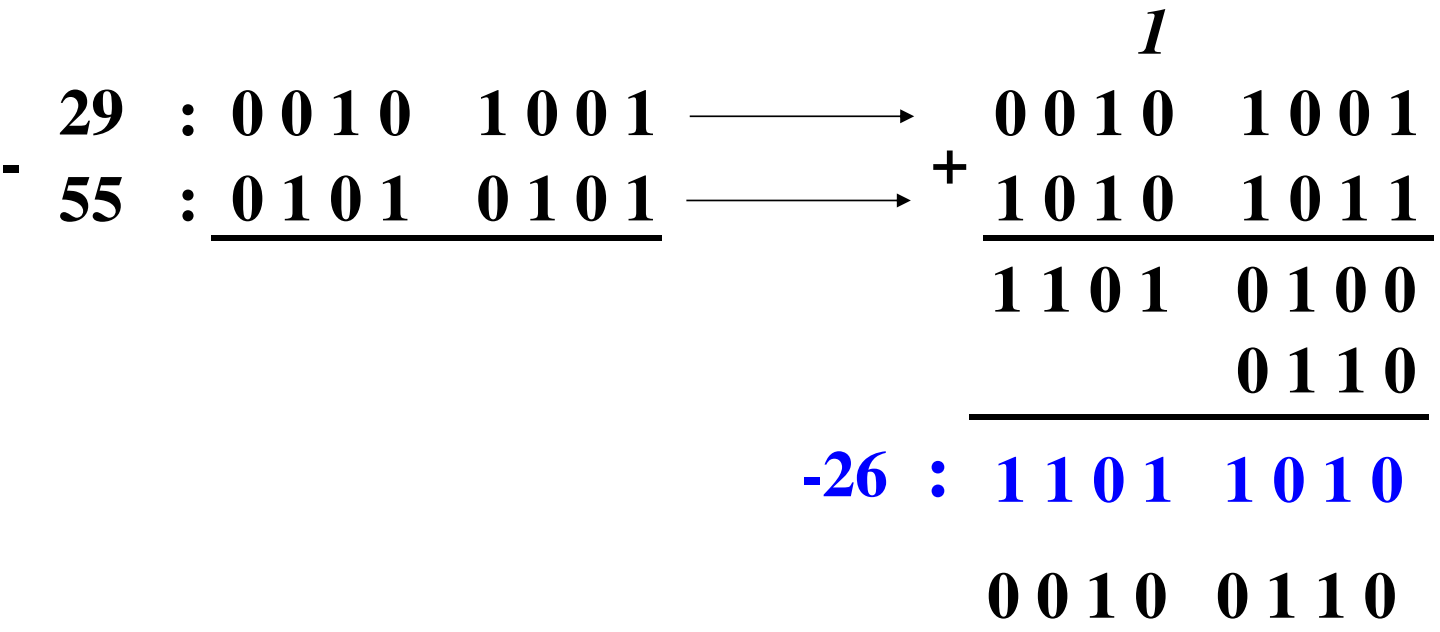
\includegraphics[width = 0.7\textwidth]{./local/image/15.png}
\end{center}